\chapter{Digital electronics and machine architecture}

\section{Introduction}

\begin{figure}
    \centering
    \includegraphics[width = 0.7\textwidth]{images/von_neumann.png}
    \label{fig:von_neumann}
    \caption{Von Neumann architecture scheme.}
\end{figure}

\begin{definition}[Von-Neumann architecture]
    \label{def:von_neumann}
    The \textbf{von Neumann architecture} is a fundamental computer architecture, the schema is shown in Figure \ref{fig:von_neumann}. It consists of
    \begin{enumerate}
        \item a processing unit that contains the arithmetic logic unit and processor registers;
        \item a control unit;
        \item a memory unit that stores data and instructions;
        \item external mass storage; and
        \item input and output mechanisms. 
    \end{enumerate}
    There is a data bus and an instruction in between the memory unit and processing unit.
\end{definition}

\begin{definition}[Little man computer]
    The \textbf{little man computer} (LMC) is a simplified model of the von Neumann architecture. It consists of
    \begin{enumerate}
        \item 100 `mailboxes' that each have a unique 2 digit address, each mailbox can store 3 digit numbers;
        \item a calculator that can display up to 3 digits, perform the addition and subtraction, and has a flag for a negative result;
        \item a 2 digit counter called the program counter; and
        \item input and output trays to allow users to input data and receive an output.
    \end{enumerate} 
    To execute an instruction, the `little man' retrieves the data stored in the data address specified by the program counter and increments the program counter by then decodes the data and performs the according instruction.
\end{definition}

\begin{definition}[Little man computer instruction set]
    A LMC instruction is split into to parts, the first digit it the \textbf{opcode} and the second and third digit is the \textbf{operand}. The opcode dictates what the instruction will do and the operand dictates the address (mailbox number) of the data of which the instruction will be applied to. The following are opercodes in LMC:
    \begin{enumerate}
        \item \textbf{LDA}, opcode 5: this will go to the mailbox specified and load the data into the calculator;
        \item \textbf{STA}, opcode 3: this will take the data in the calculator and store it into the mailbox specified, overwriting any value currently there;
        \item \textbf{ADD}, opcode 1: this will go to the mailbox specified and add it to the value in the calculator;
        \item \textbf{SUB}, opcode 2: this will go to the mailbox specified and subtract it from the value in the calculator;
        \item \textbf{INP/OUT}, opcode 9: operand 01 inputs data from the user, operand 02 outputs data to the user;
        \item \textbf{HLT}, opcode 0: the program stops.
    \end{enumerate}
\end{definition}

\begin{example}[Addition of two numbers in little man computer]
    The following LMC code will take two numbers from the user and output the addition of both of them (not accounting for overflow).
    \begin{center}
        \normalfont
        \ttfamily
        \begin{tabular}{p{2em} p{2em}}
            INP \\
            STA & 99 \\
            INP & \\
            ADD & 99 \\
            OUT \\
            HLT \\
            DAT & 99 \\
        \end{tabular}
    \end{center}
    Note that the \texttt{DAT} command flags the corresponding mailbox as data. Converting the instruction to opcodes we get the (fairly unreadable) code as follows.
    e user and output the addition of both of them (not accounting for overflow).
    \begin{center}
        \normalfont
        \ttfamily
        \begin{tabular}{p{2em}}
            901 \\
            399 \\
            901 \\
            199 \\
            902 \\
            000 \\
        \end{tabular}
    \end{center}
\end{example}

\begin{definition}[Extended little man computer instruction set]
    The original instruction set is not enough to make complex programs, here we introduce branch instructions to allow us to loop.
    \begin{enumerate}
        \item \textbf{BRA} opcode 6: sets the program counter to the specified mailbox address;
        \item \textbf{BRZ} opcode 7: sets the program counter to the specified mailbox address if the calculator holds the value 0; and
        \item \textbf{BRP} opcode 8: sets the program counter to the specified mailbox address if the calculator value is non-negative.
    \end{enumerate}
\end{definition}

\begin{example}[Output the smaller of two numbers]
    The following LMC will take two numbers from the user and output the smaller of the two.
    \begin{center}
        \normalfont
        \ttfamily
        \begin{tabular}{p{1em} p{2em} p{2em}}
            00 & INP \\
            01 & STA & 99 \\
            02 & INP \\
            03 & SUB & 99 \\
            04 & BRP & 08 \\
            05 & LDA & 99 \\
            06 & OUT \\
            07 & HLT \\
            08 & ADD & 99 \\
            09 & OUT \\
            10 & HLT \\
        \end{tabular}
    \end{center}
    Converting the instructions to opcodes we get the following code.
    \begin{center}
        \normalfont
        \ttfamily
        \begin{tabular}{p{1em} p{2em}}
            00 & 901 \\
            01 & 399 \\
            02 & 901 \\
            03 & 299 \\
            04 & 808 \\
            05 & 599 \\
            06 & 902 \\
            07 & 000 \\
            08 & 199 \\
            09 & 902 \\
            10 & 000 \\
        \end{tabular}
    \end{center}
\end{example}

\begin{definition}[Fetch-execute cycle in little man computer]
    To execute code LMC follows a fetch-execute cycle. 
    \begin{enumerate}
        \item Fetch, the `little man' fetches the instruction held in the value of the program counter and decodes the instruction.
        \item Execute, the `little man' will execute the decoded instruction, this may involving fetching data and bringing it to the calculator.
    \end{enumerate}
\end{definition}

A contrasting architecture to von Neumann is Harvard architecture, this is where instructions and data are stored in separate arrays of memory. This removes functionality (at least easily) for a self-modifying program where the program can alter the instructions stored in memory as it runs.

\begin{figure}
    \centering
    \includegraphics[width = 0.7\textwidth]{images/harvard.png}
    \label{fig:harvard}
    \caption{Harvard architecture scheme.}
\end{figure}

\begin{definition}[Harvard architecture]
    The \textbf{Harvard architecture} is another fundamental computer architecture, the schema is shown in Figure \ref{fig:harvard}. It consists of mainly the same components as the von Neumann architecture (Definition \ref{def:von_neumann}); however, the stored program and data and stored in separate arrays of memory. 
\end{definition}

Benefits for the Harvard architecture over the von Neumann architecture are as follows:
\begin{enumerate}
    \item quicker to execute as data fetching and instruction fetching can be pipelined;
    \item simpler to analyse and follow code; and
    \item avoids bugs due to self-modifying code, self-modifying code.
\end{enumerate}

\begin{example}[Calculate integer division in little man computer]

\end{example}

\begin{example}[Euclid's algorithm]

\end{example}

\section{Microarchitecture}

\begin{figure}
    \centering
    \makebox[\textwidth]{
        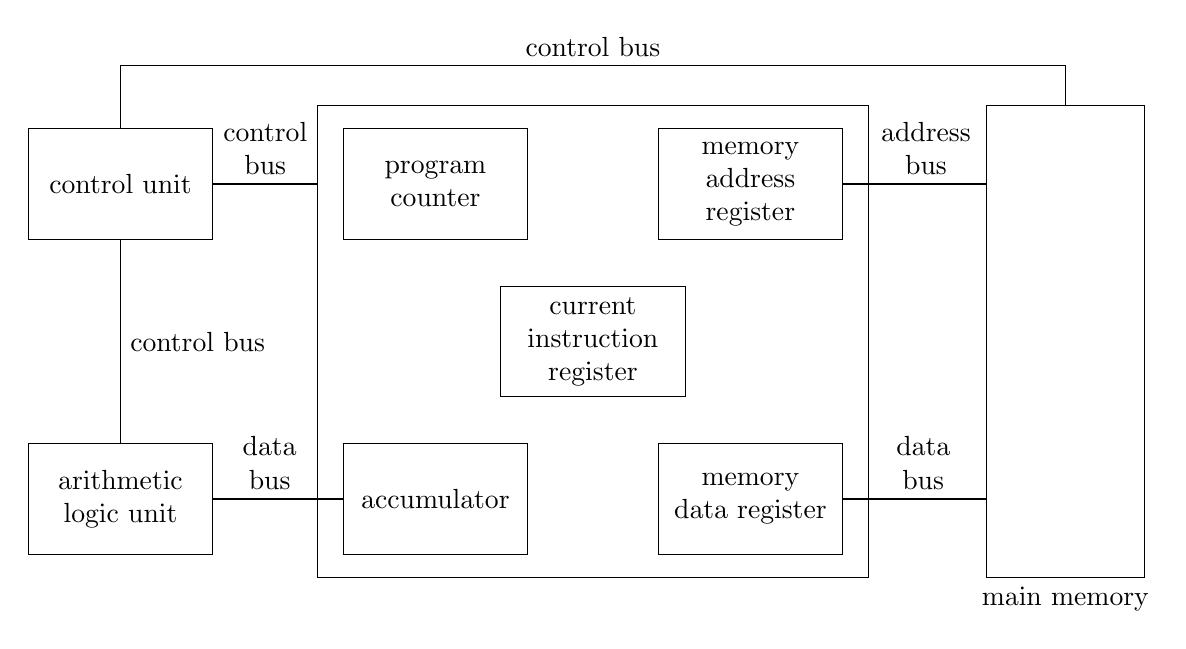
\begin{tikzpicture}
            \tikzstyle{box} = [rectangle, draw = black, text width = 6em, minimum width = 6em, minimum height = 4em, align = center]
            \node[box] at (0, 0) (alu) {arithmetic logic unit};
            \node[box] at (0, 4) (cu) {control unit};
            \node[box] at (4, 0) (acc) {accumulator};
            \node[box] at (4, 4) (pc) {program counter};
            \node[box] at (8, 0) (mdr) {memory data register};
            \node[box] at (8, 4) (mar) {memory address register};
            \node[box] at (6, 2) (cir) {current instruction register};
            \node[below] at (12, -1) {main memory};
            \draw (11, -1) rectangle (13, 5);
            \draw (2.5, -1) rectangle (9.5, 5);
            \draw (cu) -- (0, 5.5) -- node[above] {control bus} (12, 5.5) -- (12, 5);
            \draw (cu) -- node[right] {control bus} (alu);
            \draw (cu) -- node[above, align = center] {control \\ bus} (2.5, 4);
            \draw (alu) -- node[above, xshift = -3pt, align = center] {data \\ bus} (acc);
            \draw (mdr) -- node[above, xshift = 3pt, align = center] {data \\ bus} (11, 0);
            \draw (mar) -- node[above, xshift = 4pt, align = center] {address \\ bus} (11, 4);
        \end{tikzpicture}
    }
    \label{fig:basis_cpu}
    \caption{A basic processor architecture.}
\end{figure}

\begin{definition}
    A \textbf{central processing unit} (\textbf{CPU}) carries out the instructions on computer programs by performing basic arithmetic, logical, control and input/output (I/O) operations specified by the instructions. There are five major components of the CPU in relation to the little man computer model:
    \begin{enumerate}
        \item memory, the mail boxes;
        \item registers, the program counter, accumulator, and the instruction register;
        \item arithmetic logic unit, the calculator;
        \item buses, paths the data travels down; and
        \item control unit, responsible for directly the flow of instructions and data.
    \end{enumerate}
    Figure \ref{fig:basis_cpu} shows a simple schematic for a CPU.
\end{definition}

\begin{definition}
    \textbf{Registers} are storage locations in the CPU, often with a defined purpose and wired to perform that purpose. It holds binary values temporarily for:
    \begin{enumerate}[label=(\roman*)]
        \item storage,
        \item manipulation, and
        \item calculation.
    \end{enumerate}
    In the little man computer model we have
    \begin{enumerate}
        \item the accumulator, considered part of the arithmetic logic unit, this holds the result of calculation;
        \item the program counter, considered part of the control unit and stores the address of the next instruction to be fetched then executed;
        \item the instruction register, considered part of the control unit and holds the address of the current instruction being executed;
        \item the memory address register (MAR), holds the address of the data currently being accessed; and
        \item the memory data register (MDR), holds the data that has been retrieved from memory from the memory address is the MAR.
    \end{enumerate}
\end{definition}

\begin{definition}[Buses]
    Buses are simply wires that transfer data (or power) from one location to another. Buses are used to transfer data to different locations in the CPU, from CPU to memory (and vice versa), and from peripherals to the CPU. We can divide buses into four different catergories:
    \begin{enumerate}
        \item data;
        \item address;
        \item control; and
        \item power.
    \end{enumerate}
    It is clear from the categories what each type of bus transfers. We can also differentiate buses by the amount of devices receiving or sending the data:
    \begin{enumerate}
        \item point-to-point, transfers data from a specific location to a specific destination;
        \item broadcast, transfers data from a specific location to many different destination; and
        \item bus interface bridges, allows communications between different bus systems (USB is a common type of bus which differs from the buses you will find in the CPU).
    \end{enumerate}
\end{definition}

\begin{remark}
    In the little man computer model, we handle with base-10 numbers; however, in a real CPU we deal with binary. We will look at the next section how to deal with binary numbers.
\end{remark}
